% Figura 4 — Gaps principais entre o Artigo e o NOC Lite
% Fonte: artigo.tex (Sec. Taxonomia de Gaps, tab:gaps). GAP-1 a GAP-7.
% Corrigido (Chris): reconciliado com o artigo (tab:gaps) — agora desenha os 7
% gaps (GAP-1..GAP-7); "100%" corrigido para "100\%"; text width + align=center
% para evitar estouro de borda em GAP-6.
\documentclass[tikz,border=4pt]{standalone}
\usepackage{tikz}
\usetikzlibrary{arrows.meta,positioning,decorations.pathreplacing}
\begin{document}
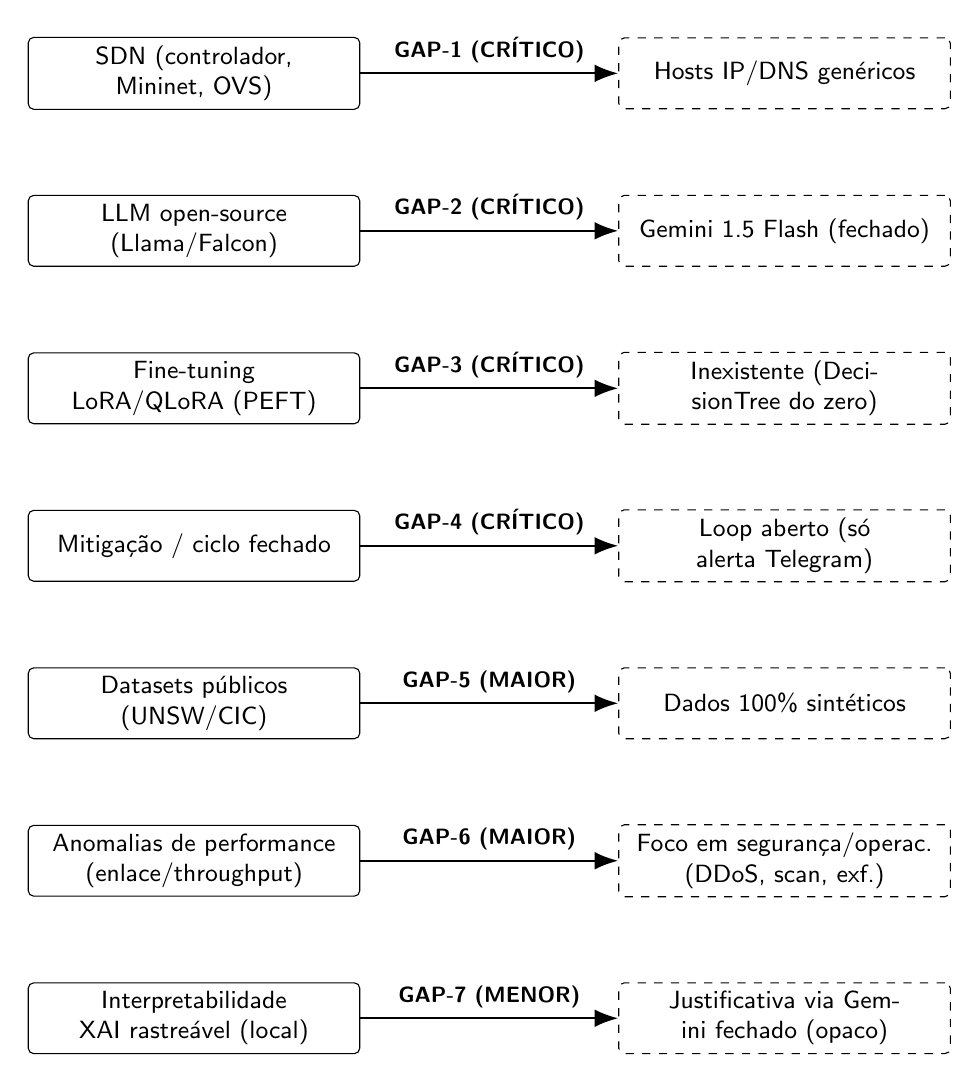
\begin{tikzpicture}[
    font=\sffamily\small,
    want/.style={rectangle, draw=black, rounded corners=2pt,
                 minimum width=4.2cm, minimum height=0.9cm,
                 text width=4.0cm, align=center, fill=white, inner sep=3pt},
    got/.style={rectangle, draw=black, dashed, rounded corners=2pt,
                minimum width=4.2cm, minimum height=0.9cm,
                text width=4.0cm, align=center, fill=white, inner sep=3pt},
    sev/.style={font=\sffamily\bfseries\footnotesize},
    arrow/.style={-{Latex[length=3mm]}, thick, draw=black},
  ]

  \node[want] (w1) at (0,12.0) {SDN (controlador, Mininet, OVS)};
  \node[got]  (g1) at (7.5,12.0){Hosts IP/DNS genéricos};

  \node[want] (w2) at (0,10.0) {LLM open-source (Llama/Falcon)};
  \node[got]  (g2) at (7.5,10.0){Gemini 1.5 Flash (fechado)};

  \node[want] (w3) at (0,8.0) {Fine-tuning LoRA/QLoRA (PEFT)};
  \node[got]  (g3) at (7.5,8.0){Inexistente (DecisionTree do zero)};

  \node[want] (w4) at (0,6.0) {Mitigação / ciclo fechado};
  \node[got]  (g4) at (7.5,6.0){Loop aberto (só alerta Telegram)};

  \node[want] (w5) at (0,4.0) {Datasets públicos (UNSW/CIC)};
  \node[got]  (g5) at (7.5,4.0){Dados 100\% sintéticos};

  \node[want] (w6) at (0,2.0) {Anomalias de performance (enlace/throughput)};
  \node[got]  (g6) at (7.5,2.0){Foco em segurança/operac. (DDoS, scan, exf.)};

  \node[want] (w7) at (0,0.0) {Interpretabilidade XAI rastreável (local)};
  \node[got]  (g7) at (7.5,0.0){Justificativa via Gemini fechado (opaco)};

  \draw[arrow] (w1) -- node[above,sev] {GAP-1 (CRÍTICO)} (g1);
  \draw[arrow] (w2) -- node[above,sev] {GAP-2 (CRÍTICO)} (g2);
  \draw[arrow] (w3) -- node[above,sev] {GAP-3 (CRÍTICO)} (g3);
  \draw[arrow] (w4) -- node[above,sev] {GAP-4 (CRÍTICO)} (g4);
  \draw[arrow] (w5) -- node[above,sev] {GAP-5 (MAIOR)} (g5);
  \draw[arrow] (w6) -- node[above,sev] {GAP-6 (MAIOR)} (g6);
  \draw[arrow] (w7) -- node[above,sev] {GAP-7 (MENOR)} (g7);
\end{tikzpicture}
\end{document}
